\hypertarget{SH__ClientCreation_8cpp}{\section{Référence du fichier logic/\-S\-H\-\_\-\-Client\-Creation.cpp}
\label{SH__ClientCreation_8cpp}\index{logic/\-S\-H\-\_\-\-Client\-Creation.\-cpp@{logic/\-S\-H\-\_\-\-Client\-Creation.\-cpp}}
}
{\ttfamily \#include $<$Q\-Regular\-Expression$>$}\\*
{\ttfamily \#include \char`\"{}S\-H\-\_\-\-Client\-Creation.\-h\char`\"{}}\\*
{\ttfamily \#include \char`\"{}S\-H\-\_\-\-Database\-Content\-Question\-State.\-h\char`\"{}}\\*
{\ttfamily \#include \char`\"{}S\-H\-\_\-\-String\-Question\-State.\-h\char`\"{}}\\*
{\ttfamily \#include \char`\"{}S\-H\-\_\-\-File\-Selection\-State.\-h\char`\"{}}\\*
{\ttfamily \#include \char`\"{}S\-H\-\_\-\-Reg\-Exp\-Question\-State.\-h\char`\"{}}\\*
{\ttfamily \#include \char`\"{}S\-H\-\_\-\-Address\-Creation.\-h\char`\"{}}\\*
Graphe des dépendances par inclusion de S\-H\-\_\-\-Client\-Creation.\-cpp\-:
\nopagebreak
\begin{figure}[H]
\begin{center}
\leavevmode
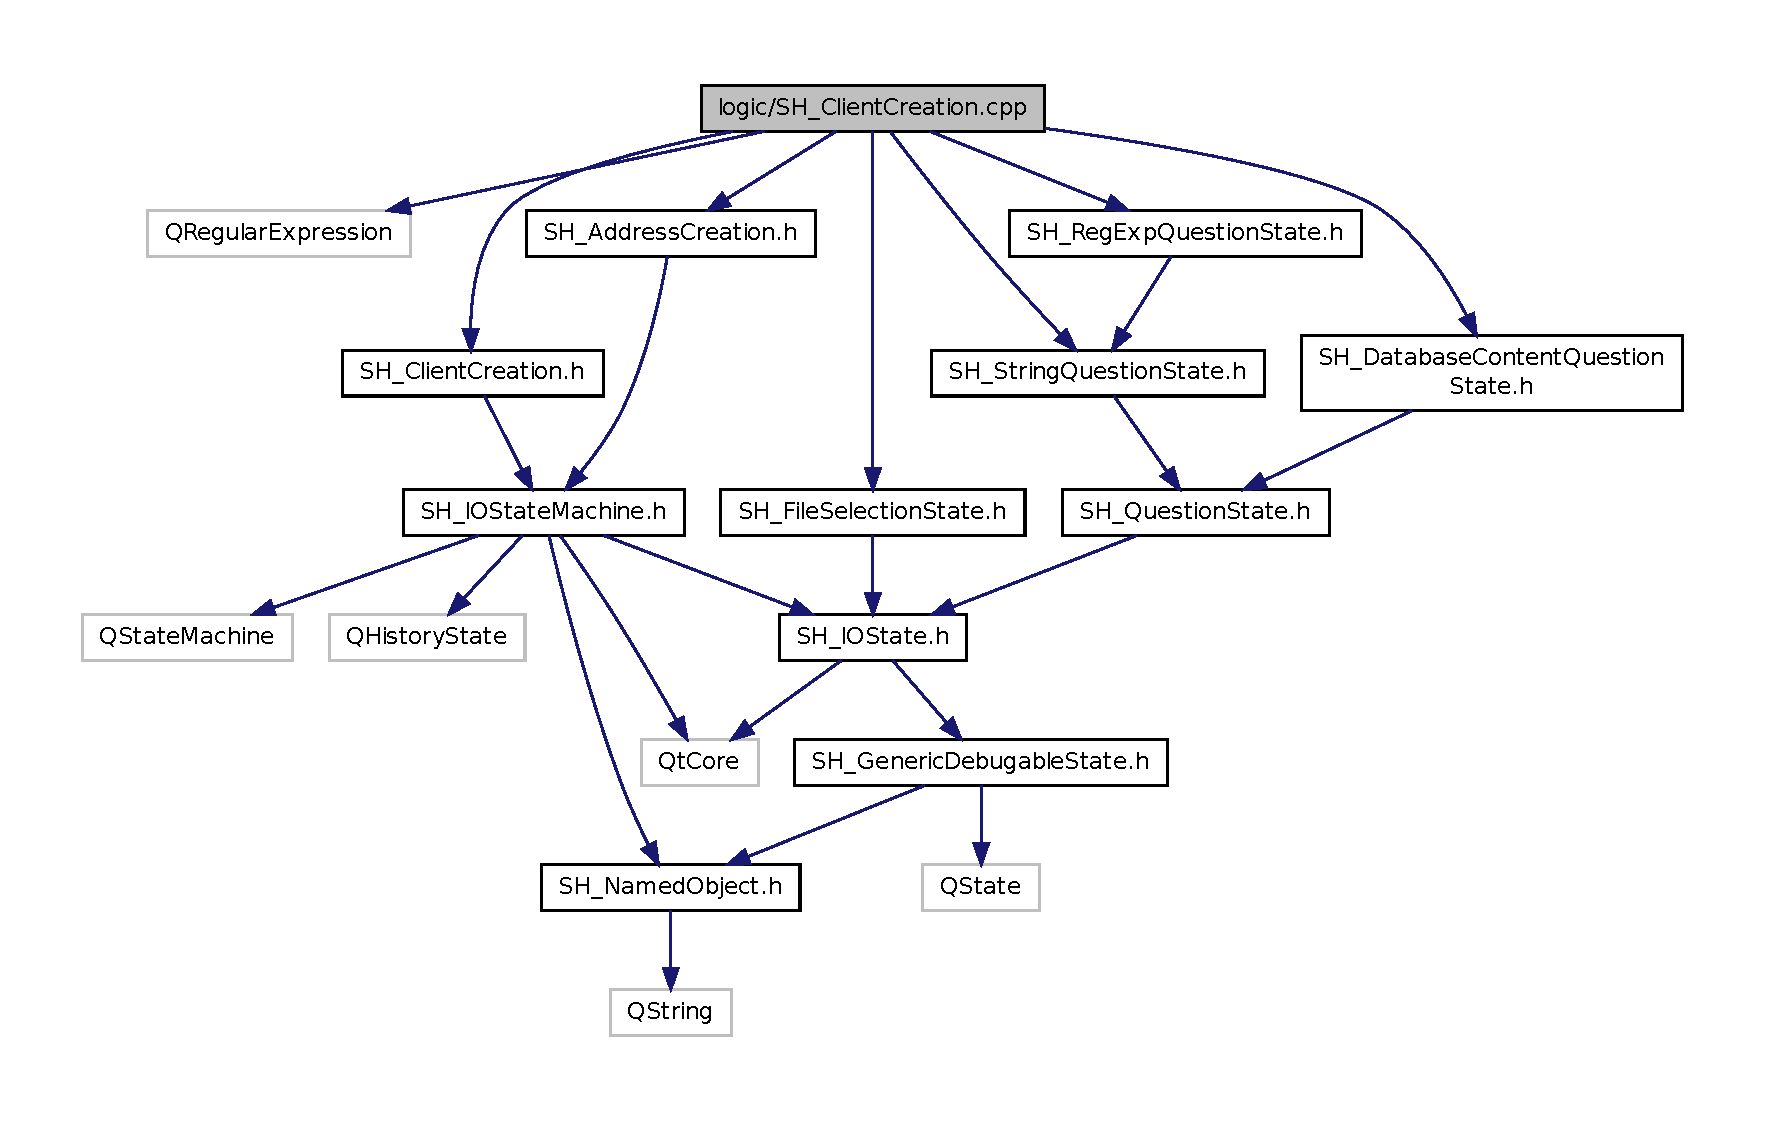
\includegraphics[width=350pt]{SH__ClientCreation_8cpp__incl}
\end{center}
\end{figure}
